\section{Empirical Validation}\label{sec:user_evaluation}
We evaluate two aspects of Algorithm~\ref{alg:constrained_alg}. First, we show that it finds a good representation for the true change points in a synthetic dataset. Second, we implement two experiments to test whether the inferred periods are interpretable by independent human validators. The first of these experiments aims to verify the salience of the inferred change points within the context of CW. The second experiment is to verify the intelligibility of the automatically generated descriptions for the inferred periods. Due to the tightly coupled relationship between the period boundaries and the regime specific parameters, separating these two factors for comparison is exceedingly difficult. However, between the two experiments, we evaluate the interpretability of the joint inference over the periods and the associated regime parameters. The evaluations suggest that the proposed techniques produce results that do have interpretabilty in the CW domain.

\section{Evaluation on Synthetic Data}

\begin{equation}
  \begin{split}
      \mathbf{X^{(1)}_t} = 0.99 \,\mathbf{X_{t-1}} + w^{(1)}_t \hspace{10pt} & w^{(1)}_t \sim \mathcal{N}(0,1) \\
      \mathbf{X^{(2)}_t} = 0.9 \,\mathbf{X_{t-1}} + w^{(2)}_t \hspace{10pt} & w^{(2)}_t \sim \mathcal{N}(0,10) \\
      \mathbf{Y_t} = S_t\mathbf{X_t} + v_t \hspace{10pt} & v_t \sim \mathcal{N}(0,0.1)
  \end{split}\label{eq:switching_state_space_results}
\end{equation}

Equation~\ref{eq:switching_state_space_results}, an adapted model from \citet{ghahramani2000variational}, describes a SSSM with two regimes and a continuous state space\footnote{The \citet{ghahramani2000variational} model describes a state space that is disjoint at regime switches. We choose to make the state space continuous at the switch points as this more accurately mimics the scenario that is present in CW.}. The transition parameters and noise are regime dependent with $A^{(1)}~=~0.99$, $A^{(2)}~=~0.9$, $Q^{(1)}~=~1$ and $Q^{(2)}~=~10$. $S_t$ is the categorical switching variable that chooses between the two regimes at every time step. The prior probability\footnote{$P(S_1=1)=p_1=P(S_1=2)=p_2=0.5$} of each of the regimes is 0.5 and the transition probabilities are $\Phi_{1,1} = \Phi_{2,2} = 0.95$ and $\Phi_{1,2} = \Phi_{2,1} = 0.05$. This model was used to generate 1000 time series, each with 200 observations.

Figure~\ref{fig:result_generated_time_series_with_labels} shows an example of a generated time series. The switch points are shown according to the true model (top), the inferred labels from Algorithm~\ref{alg:constrained_alg} (middle) and the Gaussian merging baseline (bottom). Each period is represented by a sequence of black and gray colored circles. Note that qualitatively it is a challenging task to distinguish between the regime labels by merely observing the time series values. As shown in Figure~\ref{fig:result_generated_time_series_with_labels}, the periods inferred by both Algorithm~\ref{alg:constrained_alg} and the baseline overlap to some extent with the true periods. However, there is substantially more noise (high frequency switches) in the inferred periods of the baseline.

\begin{figure}
\centering
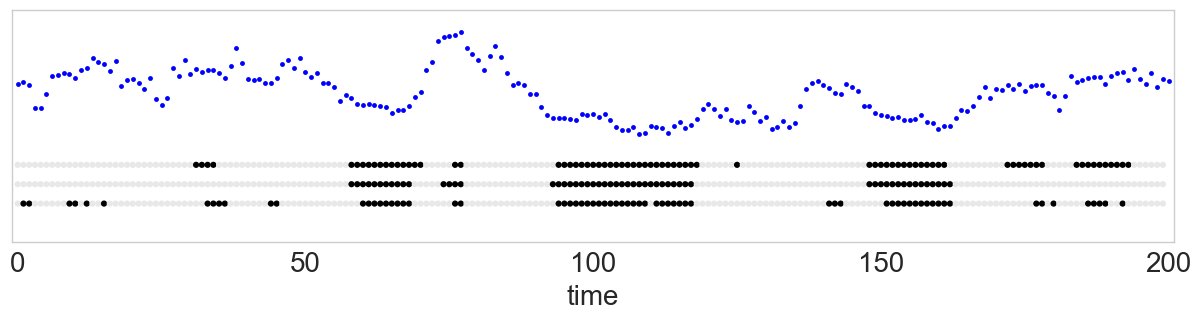
\includegraphics[width=\textwidth]{time_series_comparison.png}
\caption{An example of a generated time series from the SSSM model of equation~\ref{eq:switching_state_space_results}. The $x$ axis represents time, and the $y$ axis shows the observations. Regime labels are shown as black and gray dots representing the two label options. True labels (top) are compared to the inferred labels from Algorithm~\ref{alg:constrained_alg} (middle) and the Gaussian merging (bottom).}
\label{fig:result_generated_time_series_with_labels}
\end{figure}

We ran Algorithm~\ref{alg:constrained_alg} to learn the switch points on this data, setting the number of regimes to nine. The percent agreement between the inferred regime labels and the known labels presents the accuracy for each algorithm for each time series. Figure~\ref{fig:result_generated_histograms} shows a histogram of the algorithm accuracy according to Algorithm~\ref{alg:constrained_alg} ($a$) and the baseline Gaussian merging ($b$). The bi-modal and long tailed distribution for the baseline approach demonstrates its susceptibility to local optima. When this algorithm converges toward the correct labeling, it finds a similar structure to that inferred by Algorithm~\ref{alg:constrained_alg}. However, if the initialization of the optimization (chosen randomly) is poor, this algorithm can easily result in labeling all of the data as belonging to one regime or the other. The mean accuracy of Algorithm~\ref{alg:constrained_alg} was 89\%, materially higher than the 66\% achieved by the Gaussian merging approach.

\begin{figure}
\centering
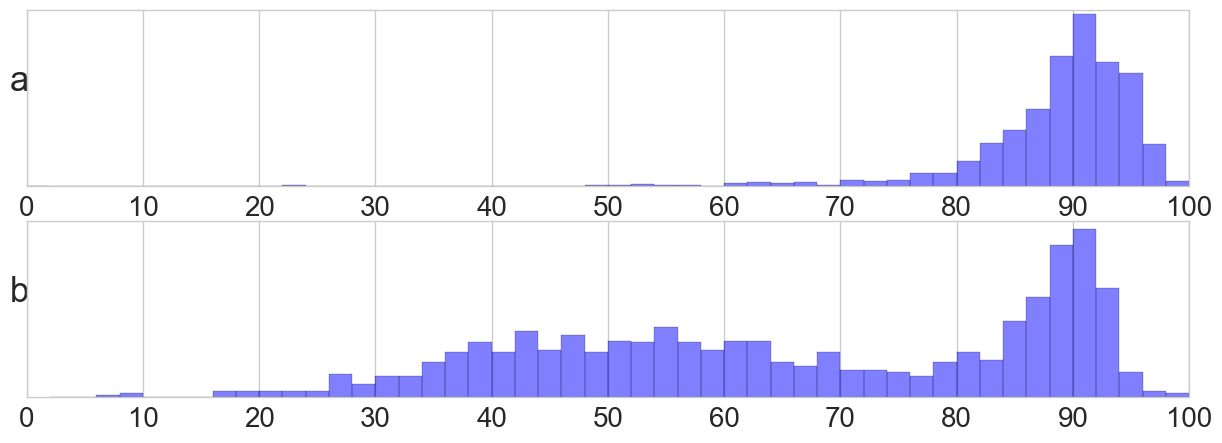
\includegraphics[width=\textwidth]{generated_results.png}
\caption{Histogram of the percent of correctly inferred labels for the observed output. The structured sampling Algorithm \ref{alg:constrained_alg} (a) learns the regime labels more accurately than the uninitialized Gaussian merging algorithm (b).}
\label{fig:result_generated_histograms}
\end{figure}

The superior performance of Algorithm~\ref{alg:constrained_alg} can be directly attributed to the switching behavior that is enforced by Assumptions 1 and 2, which was not assumed by the baseline model. Although Algorithm~\ref{alg:constrained_alg}'s model structure encourages the discovery of switches, the uniformly spaced initialization of labels should not be seen as an advantage as no prior knowledge of the actual switches is used in performing this step. The justification for enforcing a static number of switches is from Assumption 2 where the goal is to find more stable regimes and thus a lower frequency of switches between regimes. An implementation note is that although Algorithm~\ref{alg:constrained_alg} searches for $9$ regimes in the data, we know that only two are present. The presence of two regimes can be specified in the hierarchical structure of the model such that each of the 9 regimes draws its parameters from only two options. The number of regimes for the Gaussian merging approach is merely set to two.

\section{Validation of Model Interpretability}

The inference from Algorithm~\ref{alg:constrained_alg} aims to assist teachers when leading their students through a review discussion of a particular simulation session. Thus we aim to validate that the inferred switch points are interpretable to a human seeking to understand the ``story'' of the simulation. The relative magnitudes of the inferred regime parameters are used to generate a short description for the water flows for each period. The CW system provides a video representation of the log positions and the resulting water flow in the simulation. See Figure~\ref{fig:connected_worlds_graphic} for one frame from the video visualization that shows the biome positions, a distribution of logs on the floor of the simulation and the resulting flow of water at that time step. This video representation was presented to human validators to verify the change points (presented in Section~ \ref{sec:experiment1-empirical-validation}) that are found by Algorithm~\ref{alg:constrained_alg} and to verify the intelligibility (presented in Section~\ref{sec:experiment2-empirical-validation}) of the automatically generated descriptions for the inferred periods.

\subsection{Experiment 1}\label{sec:experiment1-empirical-validation}

We designed an experiment\footnote{Available at \url{http://essil-validation.s3-website-us-east-1.amazonaws.com/}} that asked evaluators to select one of three possible switch points between every pair of consecutive periods. Evaluators saw a composite of 1) the movie of the two periods; 2) a description of the dynamics of each of the two periods (e.g., ``water flows to the Desert and Plains'') and 3) a set of three possible switch points between the periods. The evaluator's task was to choose the switch point that best matched the change in dynamics between the two periods. One of the three switch points was that inferred by Algorithm~\ref{alg:constrained_alg}; the other two were random times sampled uniformly from the beginning of the first period to the end of the second period with the constraint that any two presented times cannot be within $10s$ of one another.

Evaluators worked with five sessions, each of which included $8$ to $12$ periods of system dynamics. Selecting the correct switch point is not a trivial task: it requires distinguishing between the changes in the system that indicate different dynamic regimes from the changes that are noise within the same dynamic regime. We see an evaluator's ability to choose a switch point, based on the movie and a description of the two contiguous periods, as evidence that the inferred periods are potentially useful to a teacher who wants to guide students in constructing a causal description of their experience with the simulation.

\subsection{Experiment 1 Results}\label{sec:experiment1-empirical-validation-results}

Figure~\ref{fig:results_expert_validation} presents the results of the validation using four evaluators with knowledge of the CW domain. The five sessions are shown along the x-axis; the fraction of correctly selected switch points is shown by the bin heights. The dashed line represents a random baseline in which the selected switch probability corresponds to $\frac{1}{3}$. Under the null hypothesis, the performance of an evaluator would not be significantly different than the random baseline. The results indicate that the evaluators chose the switch point identified by Algorithm~\ref{alg:constrained_alg} significantly more often than the random baseline ($p < 1\times 10^{-4}$). This suggests that the inferred switch points were, indeed, interpretable to a large extent as meaningful changes in the state of the system. The differences in interpretability seen in Figure~\ref{fig:results_expert_validation} (e.g. Session 4 was more difficult to interpret than Session 3) can provide a direction for further investigate in how to support teachers and students in making sense of their experiences in CW. For example Appendix~(TODO) presents a brief investigation into the file specific difficulties.

\begin{figure}
\centering
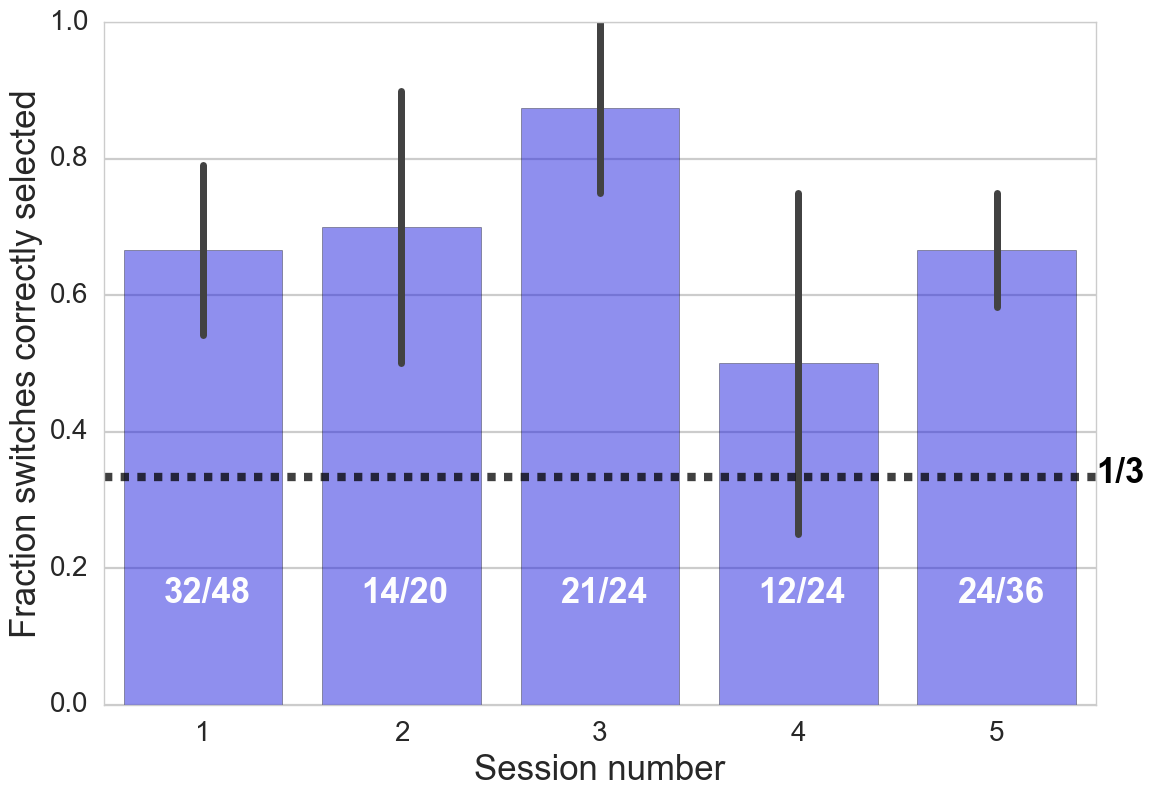
\includegraphics[width=10cm]{expert_validation_result.png}
\caption{Expert validation of five different test files from sessions with CW. The bar plot shows the fraction of correctly identified switches between automatically identified periods.}
\label{fig:results_expert_validation}
\end{figure}

\subsection{Experiment 2}\label{sec:experiment2-empirical-validation}

Experiment 2 aims to test the interpretability of the automatically generated regime descriptions when presented alongside the associated period clip from the video representation of the students' work. Validators are asked to choose one of three plausible descriptions for the dynamics that are displayed in the video clip of the period. Experiment 2 further introduces a control condition where the change points in the time series are pre-defined and the descriptions are generated, conditioned on the pre-defined change points.

Figure~\ref{fig:user_experiment_overview} shows a screen-shot of the visualization\footnote{Available at \url{https://essil-validation.herokuapp.com/}} that the users are given. Label (1) shows the video clip; this clip is played for the duration of an inferred period. Label (2) indicates one of three descriptions that might be associated with the video clip. Validators are asked to watch the video and select the description that most accurately describes the dynamics in the video for the period. The dummy descriptions for each period are randomly generated.

\begin{sidewaysfigure}
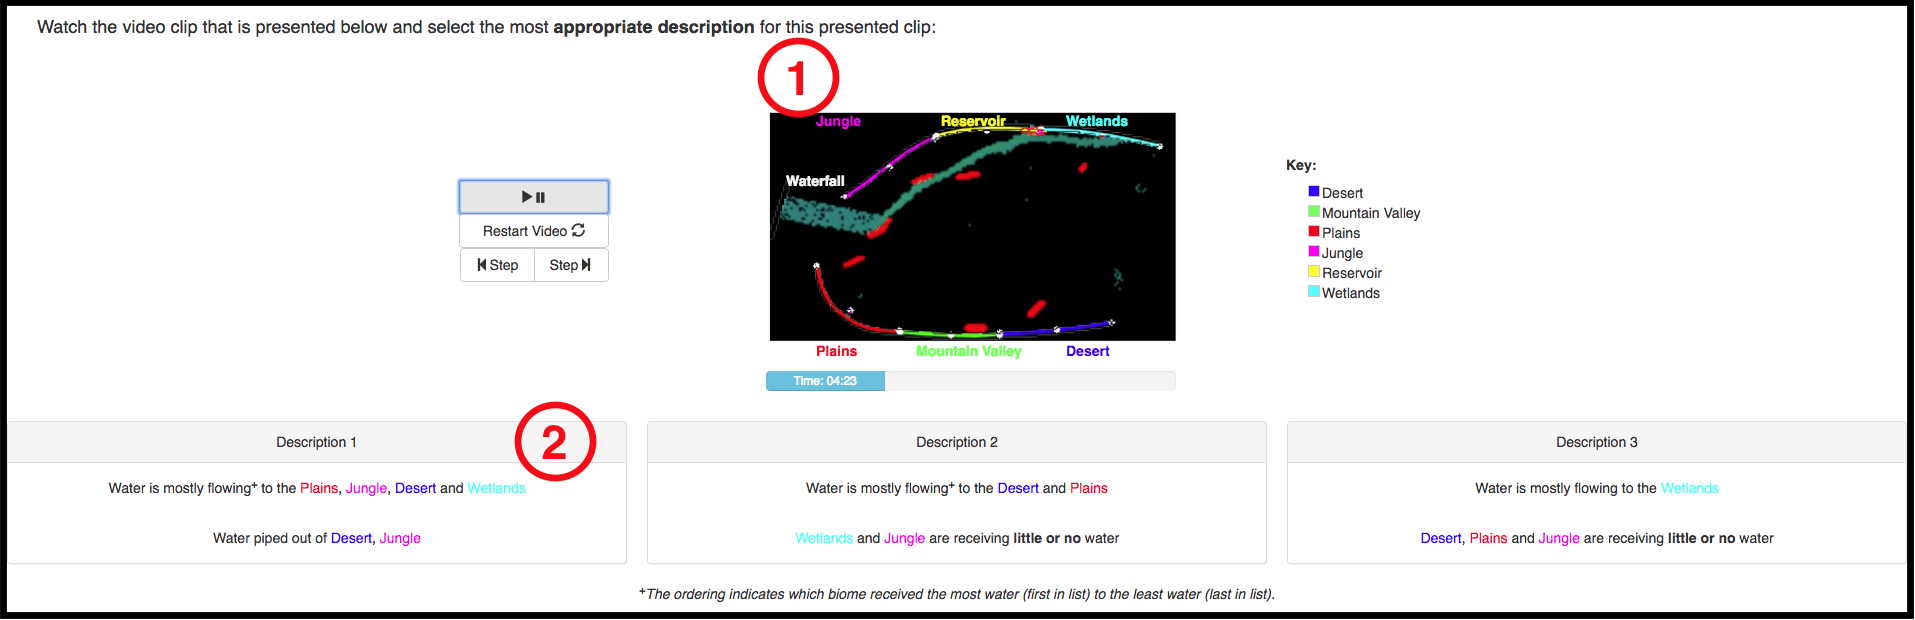
\includegraphics[width=\textwidth]{user_experiment_overview.png}
\caption{Screen-shot of the user interface designed to evaluate the interpretability of Algorithm~\ref{alg:constrained_alg}. The video representation at (1) is played for the duration of the period. Three plausible descriptions (of which (2) is one of these) are presented and the validator is asked to select the description that best describes the dynamics shown in the video. In this case, \textit{Description 3} is the correct solution.}
\label{fig:user_experiment_overview}
\end{sidewaysfigure}

The control condition in this experiment is to compare the algorithmically inferred period boundaries with boundaries that are uniformly spaced over the duration of the time series. We return to the hypothesis that deconstructing the time series into smaller periods will improve the period interpretability as the complexity of the period must decrease for shorter period lengths. Allowing Algorithm~\ref{alg:constrained_alg} to define the period boundaries should assist in finding periods that are more coherent for the associated descriptions. The algorithmically inferred periods should therefore be easier to identify than the periods that are defined uniformly across the time series.

The visualization (represented by the screen-shot in Figure~\ref{fig:user_experiment_overview}) was presented to $40$ independent validators. Each participant had little or no prior knowledge about CW. A short tutorial of $14$ slides introduces the objective for validation and explains the key aspects of the video. The participants are shown $8$ randomly selected periods from the control and the test groups. The validators are required to watch the video associated with the period and thereafter to select the description that most accurately describes the water dynamics. The results from Experiment 2 are given in Section~\ref{sec:experiment2-empirical-validation-results}.

\subsection{Experiment 2 Results}\label{sec:experiment2-empirical-validation-results}

$40$ validators independently labeled $296$ periods. The periods were generated from the same 5 session files that were presented in Section~\ref{sec:experiment1-empirical-validation}. The five files respectively had $12$,$8$,$8$,$8$ and $10$ inferred periods from Algorithm~\ref{alg:constrained_alg}. The control condition was implemented with a uniform period spacing with $8$ periods and again with $5$ periods in all $5$ test files. Figure~\ref{fig:experiment2_raw_results} shows the raw accuracy that was achieved for each file, under each algorithm. It can be seen that increasing the number of periods increases the ability of the validators to select the algorithmically generated periods. As the period lengths decrease, there are less confounding dynamics in the corresponding video clip and therefore the period description should be more recognizable to the validator.

It is also interesting to note the same general structure of the bar plot (in Figure~\ref{fig:experiment2_raw_results}) as that seen in Figure~\ref{fig:results_expert_validation}, with file $3$ having the highest success rate and file $4$ having the lowest. The file appears to affect the interpretabilty of the periods in a similar manner for both experiments. This is intuitively correct as sessions where the system dynamics are more stable (possibly due to students executing fewer actions or having a simpler goal) might make for simpler and more easily understood descriptions. However, in cases where there are possibly many conflicting student agendas, the resulting dynamics might be complex and hard to interpret.

\begin{figure}
\centering
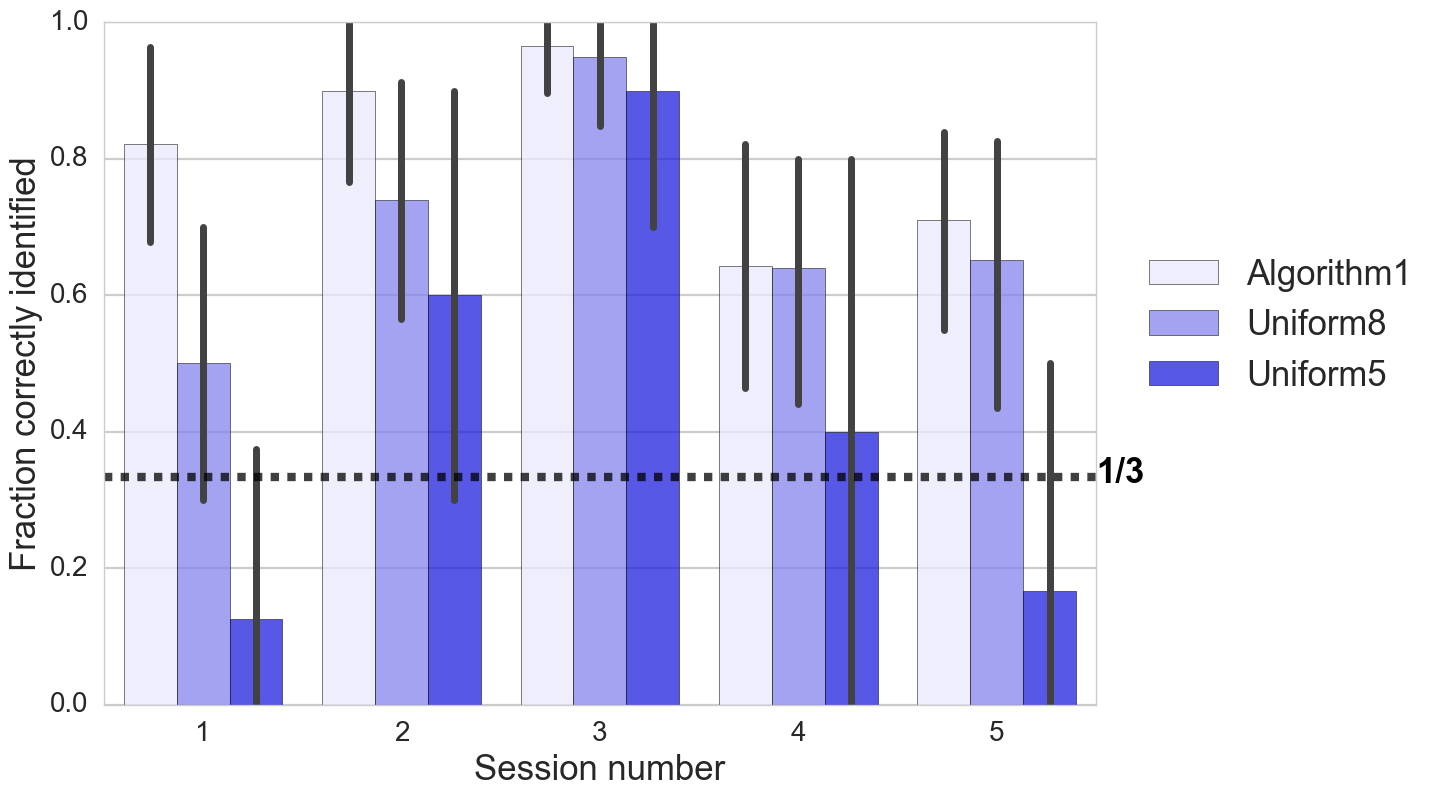
\includegraphics[width=12cm]{experiment2_raw_results.png}
\caption{Bar plot of the results from Experiment 2. There are 5 files that were tested. The fraction of correctly selected period descriptions from Algorithm~\ref{alg:constrained_alg} is compared to that from the control conditions. The control conditions include uniformly spaced periods for $8$ and $5$ periods respectively.}
\label{fig:experiment2_raw_results}
\end{figure}

\subsection{Analysis of Results for Experiment 2}
Noting that the interpretability of the periods is file specific, we design a logistic regression analysis of the results. Specifically, a hierarchical logistic regression was conducted to determine the effect of the different algorithms on the probability that a validator successfully chooses the given algorithm's generated description. We compare the effects of seeing periods and descriptions from Algorithm~\ref{alg:constrained_alg} and the control with $8$ periods (Uniform8) to the baseline of the control with 5 periods (Uniform5).

The graphical model for the hierarchical logistic regression is presented in Figure~\ref{fig:hierarchical_logistic_regression}. $\mu_f$ refers to a file specific `ease of labeling'. The Algorithm~\ref{alg:constrained_alg} and Uniform8 `interpretability effects' are added to the file specific parameter. Period specific parameters are drawn from a normal prior distribution with mean defined by the file parameter added to the effect of the algorithm used. Each period specific parameter $p_i$ represents the log-odds of a successful outcome in a Bernoulli trial. Note that the period specific parameters $p_i$ depend on the mean defined by the file and the algorithm that was used to generate the period. The variance around the file-algorithm mean is defined by the parameter $\sigma$, shared among all periods. $\sigma$ is an unknown model parameter and thus we place a weakly informative $\text{\textit{half-}}\mathcal{N}(0,1)$ prior on this parameter. We conduct inference over the algorithm interpretability effect parameters ($\alpha_a$) and the period specific log-odds parameters (presented in Appendix~\ref{cha:appendix1}).

\begin{figure}
\centering
\includegraphics[width=10cm]{hierarchical_logistic_regression.png}
\caption{Graphical model for the hierarchical logistic regression that is conducted to determine the interpretability effect of Algorithm~\ref{alg:constrained_alg} and Uniform8 over the base Uniform5 condition. The observed data $y$ corresponds to a Bernoulli trial where a description is selected to match a video clip or not. A given trial has a period specific probability of being chosen correctly $p_i$. $p_i$, in turn, depends on the file's ease of labeling and the algorithm effect. The $\alpha_a$ parameters represent the effect of the algorithm on the probability of correctly selecting the appropriate description. The periods depend on the file and algorithm means by a global variance parameter $\sigma$.}
\label{fig:hierarchical_logistic_regression}
\end{figure}

\begin{equation}\label{eq:generative_sampling_hierarchical_log}
  \begin{split}
    y_{i,k} &\mid p_i \sim Bern(logit^{-1}(p_i)) \\
    p_i &\mid \mu_f,\alpha_a,\sigma \sim \mathcal{N}(\mu_f + \mathbb{1}\{a\} \alpha_a, \sigma ) \\
    \mu_f &\sim \mathcal{N}(0,1) \\
    \sigma &\sim \text{\textit{half-}}\mathcal{N}(0,1)
  \end{split}
\end{equation}

The generative sampling distributions are given in equation~\ref{eq:generative_sampling_hierarchical_log}. The inverse logit function is used to map the real valued log-odds parameter $p_i$ to a probability between $0$ and $1$. $\alpha_a$ refers to the algorithm specific interpretability effect, with $\alpha_1$, the parameter associated with using Algorithm~\ref{alg:constrained_alg} and $\alpha_2$, the parameter associated with using Uniform8 to generate the period. $\mathbb{1}\{a\}$ is the indicator that algorithm $a$ was used to produce the description and define the duration for period $i$.

The mean posterior value for $\alpha_1 = 2.03$ with a Bayesian $95\%$ posterior confidence interval of $[1.18, 2.96]$. The value is quoted in log-odds and corresponds approximately to being $\sim 8$ times more likely that a validator will select a period correctly under Algorithm~\ref{alg:constrained_alg} than under the baseline Uniform5. This is a highly significant result suggesting that Algorithm~\ref{alg:constrained_alg} improves on the baseline Uniform5. The control group with 8 uniformly spaced periods has a posterior mean $\alpha_2 = 1.28$ (multiplicative effect of $\sim 4$ times more likely to select the period correctly over Uniform5) with a posterior confidence interval of $[0.43, 2.21]$. This too does not include $0$, the expected value for no discernible improvement, and therefore suggests that merely increasing the number of periods does help to make the periods more interpretable. However, Algorithm~\ref{alg:constrained_alg} can be compared to Uniform8 by evaluating the probability $P(\alpha_1 > \alpha_2)$. In other words, we are interested in the probability that Algorithm~\ref{alg:constrained_alg} is associated with a greater probability of choosing the generated description. This posterior probability is significant with a p-value of $p = 0.04$. The results suggest that the presented Algorithm~\ref{alg:constrained_alg} significantly improves the interpretability of the generated descriptions.

The structure of the inference executed in section~\ref{sec:experiment2-empirical-validation-results} allows us to consider the posterior probability of $p_i$ for each of the presented periods. This discussion is given in Appendix~\ref{cha:appendix1}.